\documentclass{article}

\usepackage[utf8]{inputenc}
\usepackage{amsmath}
\usepackage{amsfonts}
\usepackage{algpseudocode}
\usepackage{graphicx}
\usepackage{float}

\usepackage[style=numeric, sorting=none]{biblatex}
\addbibresource{References.bib}
\title{A Comparison of Deep Q Networks}
\author{Dylan Trollope \\\small Supervised by Prof. CJ Watkins}
\date{2022}

\begin{document}

\maketitle

\section{Abstract}
\newpage
\tableofcontents



\section{Introduction}

Reinforcement Learning (RL) is learning from interaction - a type of learning in which an agent (or learner) seeks to reach a goal state within an environment. Rather than being told which action to take, the agent discovers which action is best to take, given its current state in the environment, by maximising some reward signal or function. 

Recent advances in the field of Deep Learning have made it possible to extract high level features from high-dimensional input data, such as the creation of the convolutional neural network for image recognition and the transformer for speech recognition and language processing [references].

The fields of Deep Learning and Reinforcement Learning can be combined into a type of learning called Deep Reinforcement Learning, which has shown to give agents the ability to make decisions from large amounts of input data (such as a snapshot of an Atari game) in order to maximise their reward in order to reach a goal\cite{mnih2013atari}. 

In this report, several Deep Reinforcement Learning architectures, known as Deep Q Networks, will be implemented and compared in a number of Environments available in OpenAI's Gym library. The aim of these comparisons will be to experiment with and discuss the performance of these networks and how the properties of the Environments  contribute towards the performance of these networks.

\newpage


\section{Introduction to Reinforcement Learning}

This section introduces the main concepts and components necessary to define RL problems. 

\subsection{Components of Reinforcement Learning}

Besides the agent and environment, there are several components that make up a whole reinforcement learning problem\cite{Sutton1998}, namely: 

\begin{itemize}
    \item A Policy dictates the agent's decision-making process at any given time. A policy is roughly a function that maps perceived states in an environment to actions to be taken when in those states. Policies can range from simple functions or choosing a value from a table to more complex, computationally expensive functions that may include Neural Networks. In general a policy will, given a state, assign probabilities to the actions to take in that state. 
    
    \item A reward signal: At each time step, the environment sends the agent a reward for the action it has taken. The reward signal defines the goal of a reinforcement learning agent - the agent seeks to maximise the reward it accumulates over time.
    
    \item A value function: While the reward signal indicates what are \textit{good} actions to take in the short tern, the value function tells the agent which actions are most valuable in the long term. In RL, the value of a state estimates how much reward the agent will accumulate in the future, starting from that state. The value function takes into account the states that are most likely to follow the current state and the rewards available at those states. For example, tt is possible that a state yields a low immediate reward but offers a high value as the states that follow all yield high rewards. The reverse may also be true.
    
    Values may be seen as secondary to rewards, as without rewards there are no values to estimate but the function of the value is to achieve more reward. Yet, it is the value function that must be considered when deciding which action is best to take as this will maximise the reward the agent receives over the long run, and ultimately bring the agent closer to the goal state. It will become clear later then, that finding methods to accurately estimate the value function is crucial in succeeding in RL problems.
    
    \item Lastly, RL problems may be comprised of a model of the environment: This is used to mimic the environment the agent finds itself in and can be used to make inferences about how the environment will behave. This allows predictions to be made about the environment: given a state and an action, the model may be able to predict the next state and reward from that action. This allows the agent to \textit{plan} - the agent may be able to take a course of action made from these predictions rather than only estimating what the next best state may be.
    
\end{itemize}


\subsection{Markov Decision Process}

Markov Decision Processes (MDPs) can be used to formalise sequential decision making. 

Given a process is in a state $s$, the \textit{decision maker} within the process chooses an action $a$ that is available to it in state $s$. At the next time step, the process moves into the state, $s'$, as a result of action $a$ from the previous time step and also gives the decision maker a reward, $R_{a}(s, s')$, corresponding to its new state.

The probability that a process moves into state $s'$ is dependent on the action chosen at the previous state, and is given by the state transition function $P_{a}(s, s')$ - the current state depends on the previous state $s$ and the action $a$ taken in the previous state. 

Formally, an MDP can be defined as a 4-tuple $\langle S, A, P_a, R_a \rangle $, where: 

\begin{itemize}
    \item $S$ is the set of states - the state space
    
    \item $A$ is the set of actions - the action space, where $A_s$ is the set of actions available in state $s$.
    
    \item $P_{a}(s, s')$ is the probability that action $a$ in state $s$ will lead to state $s'$
    
    \item $R_{a}(s, s')$ is the reward received from after transitioning to state $s'$ from state $s$ after taking action $a$
\end{itemize}


\subsection{Interaction between Agent and Environment}

In RL, the agent (or \textit{learner}) is placed inside an environment, comprised of everything outside the agent. The agent selects varying actions to perform, which present new situations (or states) to the agent. Every action taken in an environment also produces a reward - a numerical value that the agent aims to maximise over time by the selecting the \textit{best} actions\cite{Sutton1998}. 

\begin{figure}
    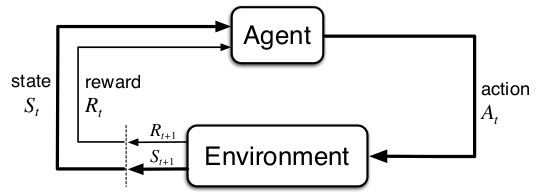
\includegraphics[scale=0.6]{images/Agent_Env_Interaction.png}
    \caption{The Agent-Environment Interaction Cycle}
    \label{fig:ag_env_interaction}
\end{figure}


Formally, the agent and environment are in interaction with each other in a sequence of (discrete) time steps, $ 0 < t < T$. At each time step, $t$, the agent receives partial (or full) information about the environment's current state, $ S_t \in \mathcal{S}$ and selects an action $a$ at time $t$ from the complete action space, $A_t \in \mathcal{A}(s)$. 

At the next time step, $t+1$, the agent receives a numerical reward as a result of the action it took at the previous time step, $R_{t+1} \in \mathcal{R} \subset \mathbb{R}$ and is then in a new state, $S_{t+1}$. 

Together, the MDP and agent-environment interaction form a sequence as follows: 

$S_0, A_0, R_1, S_1, A_1, R_2, S_2, A_2, R_3 \cdots $


\subsubsection{Rewards and Return}

Over the Reinforcement Learning process, rewards are accumulated as the agent takes actions in sequential states of the environment. These rewards can be positive or negative. 

In Environments where rewards are positive, the agent most likely aims to maximise these rewards. In Environments where the rewards are negative (also referred to as costs), the agent may seek to minimise these rewards (costs)\cite{RLNotes}.

In an MDP, the agent seeks to maximise its \textbf{return}. The return may be thought of as an \textit{average reward} over a long run of decisions. The maximisation of the return will be considered the \textit{goal} of the agent, which is a distinct feature of reinforcement learning, compared to other forms of learning.

Given that an agent receives rewards at sequential time steps, 

$R_{t+1}, R_{t+2}, R_{t+3}, R_{t+4}, \cdots, R_T$, the simplest return of the agent can be calculated as: 

\begin{equation} \label{eq:1}
\rho_{t} = R_{t+1} + R_{t+2} + R_{t+3} + R_{t+4} + \cdots + R_T
\end{equation}

This return function is used when the RL problem is episodic in nature as it expects a final state at time $T$, which is the terminal state.

As can be seen from above, the return function is linear - immediate rewards and future rewards are \textit{weighted} equivalently, there is no incentive for the agent to take actions that would maximise reward over the long run or the short run, which for certain environments may be desirable. 

By introducing a discount factor into the return function, the agent can account for maximising more immediate or future rewards\cite{RLNotes}: 

\begin{equation} \label{eq:2}
\rho_{t} = R_{t+1} + \gamma R_{t+2} +  \gamma^2 R_{t+3} + \gamma^3 R_{t+4}  + ... = \sum_{k=0}^{\infty} \gamma ^k R_{t+k+1}
\end{equation}

where $0 \leq \gamma \leq 1$ is the discount rate and determines the value of future rewards that the agent receives. If the agent receives a reward $k$ time steps in the future, it is only worth $\gamma^{k-1}$ times what it would be worth if it were received immediately.

With $\gamma$ close to 0, the agent is very short-sighted and only concerned with maximising immediate rewards - it will choose an action $A_t$ to only maximise $R_{t+1}$.

With $\gamma$ approaching 1, the return function takes future rewards into account more significantly and the agent is more farsighted. 

Using equation (\ref{eq:2}) above, it can be shown how return functions at successive time steps are related\cite{Sutton1998}\cite{RLNotes}:

\begin{align}
\rho_t &= R_{t+1} + \gamma R_{t+2} +  \gamma^2R_{t+3} + \gamma^3R_{t+4} + ... \nonumber \\
     &= R_{t+1} + \gamma (R_{t+2} + \gamma R_{t+3} + \gamma^2 R_{t+4} + ... )  \nonumber \\
     &= R_{t+1} + \gamma \rho_{t+1} 
\end{align}

$\gamma$ is used to define a \textit{soft} time horizon (Watkins, 2021). The greater the amount of time steps away from the current state, the less the return calculated from those time steps


\subsection{Policy and the Value Function}

\subsubsection{Policy}

Most RL algorithms are concerned with estimating a value function - a function that estimates how \textit{good} it is for an agent to be in a state or how \textit{good} it is to perform a given action in a given state. A state is \textit{good} if the expected reward, or more specifically, expected return from that state to the terminal state is maximised\cite{Sutton1998}. Because future expected return is dependent on the sequence of actions taken by the agent in consecutive time steps, the value function is defined in terms of the behaviour of the agent, called a \textbf{policy}.

Formally a \textbf{policy} is a function that maps states to the probability of selecting the possible actions in those states and is denoted by $\pi$. In general, RL algorithms will attempt to find the optimal policy. An optimal policy is the policy that will maximise the expected return, starting in any state.

If an agent is following policy $\pi$ at time $t$, then $\pi(a|s)$ is the probability that $A_t = a$ and $S_t = s$. The policy defines a probability distribution over $a \in A(s)$ for each $s \in S$. 

RL algorithms will specify how the agent's behaviour changes as a result of its experience.

**Deterministic vs stochastic policies and policy space**

\subsubsection{Value Function}

The value function of a state $s$ under policy $\pi$, denoted $v_\pi(s)$, is the expected return from state $s$ to the terminal state under policy $\pi$.

From the perspective of an MDP, the value function can be defined as follows\cite{RLNotes}\cite{Sutton1998}: 

\begin{align}
    v_\pi(s) &= \mathbb{E}_\pi [\rho_t | S_t = s, \pi]  \nonumber\\
             &= \mathbb{E}_\pi \left[\sum_{k=0}^{\infty} \gamma ^k R_{t+k+1}| S_t = s, \pi\right]
\end{align}subtitle
for all $s \in \mathcal{S}$, where $\mathbb{E}_\pi$ denotes the expected value of return given the agent follows policy $\pi$ at any time step $t$. 

The function $v_\pi$ is known as the \textit{state-value function}.

As will be useful later, Equation (4) can be rearranged as follows\cite{UCBSlides}: 

\begin{align}
    v_\pi(s) = R(s, \pi(s)) + \gamma \mathbb{E}_{s' \sim P(s'|s, \pi(s))} \left[ v_\pi(s')\right]
\end{align}

where the first term in the equation is the immediate reward and the second term is the return gained from the successor states when starting at state $s$ and following policy $\pi$.

\subsubsection{Q Value}

It is also possible to define the \textit{action-value function} under policy $\pi$, which is the expected return starting from $s$, taking action $a$ then continuing under policy $\pi$\cite{RLNotes}\cite{Sutton1998}:

\begin{align}
    q_\pi(s, a) &= \mathbb{E}_\pi [\rho_t | S_t = s, A_t = a, \pi]  \nonumber\\
                &= \mathbb{E}_\pi \left[\sum_{k=0}^{\infty} \gamma ^k R_{t+k+1}| S_t = s, A_t = a, \pi\right]
\end{align}

It can be seen that the summation term above is the same as the summation term in value function in Equation (4) above, i.e. The Q value can be written in terms of the value function. 

Just as Equation (4) can be rewritten in Equation (5), the equation in (6) above can be represented in the following way\cite{UCBSlides}: 

\begin{align}
    q_\pi(s,a) = R(s,a) + \gamma \mathbb{E}_{s' \sim P(s'|s, a)} \left[ v_\pi(s')\right]
\end{align}

The functions $v_\pi$ or $q_\pi$ can be estimated over time. 

Given an agent follows policy $\pi$ and maintains an average of the expected return for each state encountered, then the average return for each state will converge to that state's value $v_\pi(s)$ as the number of times it is encountered approaches infinity.

If averages are kept for each unique action taken in each state, then the averages will also converge to the expected return of the action-value function, $q_\pi$\cite{Sutton1998}.

\subsection{Optimal Polices and Value Functions}

For finite MDPs, it is possible to define precisely what it means for a policy to be optimal\cite{Sutton1998}. 

Value functions define a partial ordering over policies. A Policy $\pi$ is defined to be equal to or better than a policy $\pi'$ if its expected return is greater than or equal to that of $\pi'$ for all states:

$\pi \geq \pi'$ if and only if $v_\pi(s) \geq v_{\pi'}(s)$ for all $s \in \mathcal{S}$.

The \textit{optimal policy} is that policy which is greater than or equal to all other policies - the optimal policy is not necessarily a unique policy and is denoted by $\pi_*$. 

The optimal state-value function can be formalised as: 

\begin{align}
    v_*(s) = \underset{\pi}{\text{max}}\ v_\pi(s)
\end{align}

for all $s \in \mathcal{S}$. \\


Similarly, the optimal action-value function, $q_*$ can be formalised as: 

\begin{align}
        q_*(s, a) = \underset{\pi}{\text{max}}\ q_\pi(s, a)
\end{align}

for all $s \in \mathcal{S}$ and $a \in \mathcal{A}(s)$


\subsection{Optimality and the Bellman Equation}

A key problem to consider is exactly \textit{how} to know when a policy is optimal.

Given that the optimal policy $\pi_*$ is the policy that maximises $v_\pi(s)$ for every $s \in \mathcal{S}$, the optimal return function, also known as a Bellman equation can be defined as follows\cite{Sutton1998}:

\begin{align}
    v_*(s) &= v_{\pi_*}(s) = \underset{a}{max}(R(s, a) + \gamma \mathbb{E}_{s' \sim P(s'|s, a)} \left[ v_{\pi_*}(s')\right]) \\
    \pi_*(s) &= \underset{a}{argmax}(R(s, a) + \gamma \mathbb{E}_{s' \sim P(s'|s, a)} \left[ v_{\pi_*}(s')\right]) 
\end{align}



It is possible to define the optimal value function and optimal policy in terms of the optimal $q$ value:

From Equation (5) and Equation (10), it can be derived that:
\begin{align}
    v_* (s) = \underset{a}{max} (q_*(s, a))
\end{align}


and also from Equation (7) and (11),

\begin{align}
    \pi_*(s) = \underset{a}{argmax}(q_*(s,a))
\end{align}

These equations, known as Bellman equations, must hold for every state of the RL problem and give the conditions for a policy and its associated value function to be optimal. 

\newpage

\section{Q Learning}

Now that it has been underlined that it is possible to know that a policy is optimal, \textit{Q Learning} (Watkins 1989) is introduced as a method to calculate the optimal Q Values and subsequently the optimal policy for an RL problem\cite{Watkins:89}. As will be shown later, Q Learning will be the main algorithm built upon to perform Deep Reinforcement learning. 

Q Learning is a model-free RL algorithm that is used to learn the \textit{Q Value} of an action in a particular state. It is a model-free algorithm in the sense that:

\begin{itemize}
    \item the algorithm does not need to have a model of the environment to learn the best action to take in a given state, and 
    
    \item the algorithm can learn Q Values without knowing what the next state is, what the expected return of the subsequent states will be or what the transition probabilities from any state $s$ to $s'$ will be. 
\end{itemize}

It may seem intuitive that state transition probabilities need to be learned but this is not the case. Using Q-Learning it is possible for the agent to learn an optimal policy without ever learning state transition probabilities or expected rewards from states\cite{RLNotes}.

\subsection{Initial Setup}

The only data structure required to perform Q Learning is a table to store estimated Q values for every state and every action which is incrementally updated to approach the optimal policy.

For every state-action pair there is a $Q(s,a)$ value.

\subsection{Experience}

Q-Learning relies on episodes of experience to learn the optimal policy. 

An experience is a 4-tuple $ \langle s, a, s', r \rangle$
and describes the reward $r$ received when transitioning from state $s$ to $s'$ by taking action $a$.

\subsection{Updates}

With the Q table initialised, Q values are updated until \textit{convergence}, as follows: 

\begin{algorithmic}
    \For{each episode} 
        \State Initialise s
        \For{each step of episode}
            \State Choose $a$ from $s$ using policy from Q
            \State Take action $a$ in $s$ and observe $r$ and $s'$
            \State $Q(s,a) \gets (1 - \alpha) Q(s,a) + \alpha (r + \gamma \underset{a'}{max}Q(s', a'))$
            \State $s \gets s'$
        \EndFor
        \State Until $s$ is terminal
    \EndFor
\end{algorithmic}

\subsection{Off Policy Learning}

Q-Learning is \textbf{off policy} RL algorithm, in that it needs only the experience 4-tuple $ \langle s, a, s', r \rangle$ to learn the relevant $Q(s,a)$ values. The agent does not need sequential experiences in order to learn the optimal policy.

However, to converge to the optimal Q values, the algorithm does need to explore every combination of states and actions "repeatedly and thoroughly" (Watkins, 2021). It can be seen that Q-Learning requires very little awareness of the environment it is in and the algorithm is rather simple. All that is required is to repeatedly update the Q table using the algorithm above. 


\subsection{Converging to the Optimal Policy}

Q-Learning uses approximate value iteration to find the optimal policy. This means that the learned policy "will become arbitrarily close to the optimal policy after an arbitrarily long period of time" (Daley, 2020). Using the Bellman equation as an iterative update (defined above), the value iteration algorithm converges to the optimal action-value function, $q_t \xrightarrow[]{} q_*$ as $t \xrightarrow[]{} \infty$. For this to occur, two conditions need to be met. 

\begin{enumerate}
    \item The learning rate must approach 0. 
    
    \item Every state-action pair must be visited infinitely often. This is achieved as long as every action in a state has a non-zero probability of being selected. 
\end{enumerate}


\subsection{Exploration vs Exploitation}

In RL, the agent tends to take actions which it has tried in the past and found successful in adding maximising its Q value. But, in order to discover these state-action pairs, the agent must take actions that it has not attempted before. This means that the agent needs to \textit{exploit} what it has already learned but it also needs to explore new actions in previously unseen states in order to maximise the Q values. The problem that an RL agent faces is that if it were to only employ one strategy, it would almost certainly fall short of its goal, and so a balance between exploration and exploitation needs to be found in order to continually approach the optimal Q values and ultimately the optimal policy. 



\newpage


\section{From RL to Deep RL}

Deep Learning, a form of supervised machine learning, which uses neural networks to transform sets of (possibly high-dimensional) inputs to outputs, has shown significant progress in the fields of computer vision (such as YOLOv3 (Redmon, 2018)), natural language processing (such as BERT (Devlin et al., 2018)) and Bioinformatics in the form of AlphaFold (Jumper et al., 2021). 

\subsection{Applying Deep Learning to RL}

Using Deep Learning, agents can make decisions from large amounts of (unstructured) input data without being aware of the state space. It has been shown possible to play games like Atari Breakout to an expert level using Deep Reinforcement Learning (Mnih et al., 2013). Using a variant of Q-Learning, later described as a Deep Q Network, the model was able to learn policies directly from input data (4 consecutive frames of Breakout gameplay) using a Convolutional Neural Network and output a value function to predict future rewards. 


\subsection{Challenges to Consider when Applying Deep Learning to RL}

There are some challenges to consider in the application of Deep Neural Networks to problems that have been traditionally thought of as Reinforcement Learning Problems:

\begin{itemize}
    \item Firstly, Deep Learning (a type of \textit{supervised} learning) applications are able to find accurate, generalised models by using large volumes of hand-labelled training data. In comparison, RL algorithms tend to learn from a scalar reward function that can be \textit{noisy} and \textit{delayed} - delayed in the sense that the true reward for an action in a state may only be seen thousands of time steps after that action was taken. This type of delay does not exist in Deep Learning as, once the network is trained, there is an (almost) instant prediction between an input and its predicted label.
    
    \item Secondly, in deep learning, most networks are assumed to take as input, samples that are i.i.d (Independently and Identically Distributed). In comparison, RL encounters sequences of states that are highly correlated to each other - i.e. Getting to state $s'$ from $s$ may be completely dependent on taking action $a$. There may also be a distribution shift in the RL distribution as the algorithm learns new behaviours, which may present challenges to deep learning algorithms that assume the data distribution is fixed.
    
\end{itemize}


\subsection{Neural Network as a Function Approximator}

When outlining the conditions needed for Q-Learning to converge, it is stated that: 

$q_t \xrightarrow[]{} q_*$ as $t \xrightarrow[]{} \infty$. 


In practice however, it is impractical to use this approach as $q(s,a)$ is estimated for every sequence (episode) and so there is no generalisation between many sequences. To remedy this, a neural network with weights $\theta$ is introduced as a non-linear function approximation in order to estimate $q(s, a, \theta) \approx q_*(s,a)$. This network is known as a Q-Network (Mnih et al., 2013).  


\subsubsection{Training a Q-Network}

The Q-Network is trained by minimising a sequence of loss functions, $\mathcal{L}_i(\theta_i)$ that changes for every iteration,

\begin{align}
    \mathcal{L}_i(\theta_i) = \mathbb{E}_{s,a \sim p(s,a)} \left[ (y_i - q(s,a, \theta_i))^2 \right]
\end{align}

where 

\begin{align}
    y_i = \mathbb{E}_{s' \sim \mathcal{S}} \left[r + \gamma \underset{a'}{\text{max}}\ q(s', a', \theta_{i-1})|s,a \right]    
\end{align}

is the target for iteration $i$ and $p(s,a)$ is the probability distribution over sequences of states and actions, also known as the \textit{behaviour distribution}. The parameters of the previous iteration $\theta_{i-1}$ are kept fixed for the current iteration of the loss function $\mathcal{L}_i(\theta_i)$. It is important to note that, unlike in supervised learning where targets are fixed before learning, the targets for $\mathcal{L}_i(\theta_i)$ are dependent on the current network weights. 

Differentiating the loss function with respect to the weights, the gradient is as follows: 

\begin{align}
    \nabla_{\theta_i} \mathcal{L}_i (\theta_i) = \mathbb{E}_{s,a \sim p(s,a);s' \sim \mathcal{S}} \left[ (r + \gamma \underset{a'}{\text{max}}\ q(s', a', \theta_{i-1}) - q(s,a,\theta_i)) \nabla_{\theta_i}\ q(s,a,\theta_i) \right]
\end{align}

Because it is computationally expensive to compute the full expectations of the above equation, stochastic gradient descent can be used to optimise this loss function. If there are updates after every time step and the expectations are replaced by single samples from the behaviour distribution $p(s,a)$ and $\mathcal{S}$ respectively, we arrive at the Q-Learning algorithm (Mnih et al., 2013). 

\subsection{Model Free and Off-Policy}

Just as in Q-Learning, it is important to note that Deep Q Networks are \textit{Model Free} and  adopt \textit{Off-policy} learning.  

It is model-free in that it solves the RL problem directly by using samples from the state-space $\mathcal{S}$ without explicitly learning about the environment in which the agent is placed. It is off-policy in that it learns a \textit{greedy} strategy $a = \underset{a}{\text{max}}\ q(s,a,\theta)$ while ensuring adequate exploration of the state space. 

In practice, the behaviour distribution is selected by an $\epsilon$-greedy strategy that follows the strategy with probability 1 - $\epsilon$ and selects a random action with probability $\epsilon$.

\subsection{Experience Replay in Deep Q Networks}

Q-Learning makes use of episodes of experience, where the experience at time $t$ takes the form $e_t = \langle s, a, s', r \rangle$. 

In Deep Q Networks, we want to store these experiences $\mathcal{D} = e_1, e_2, ..., e_T$ in memory called an \textit{experience replay}. When training the Deep Q Network, the Q-Learning updates are applied to samples of the experience memory, $e \sim D$, drawn at random from the store of experiences, $\mathcal{D}$. 

Upon performing experience replay, the agent selects an action according to an $\epsilon$-greedy policy. A fixed-length history of experience is used in order to train the neural network. 

\subsubsection{Advantages of Using Randomly Sampled Experience Replay}

The Experience Replay approach described above provides some efficiencies during training: 

\begin{itemize}
    \item Each step of experience may be used in many weight updates, providing greater data efficiency
    
    \item As sequential experiences are highly correlated, using random samples ignores this correlation, reducing the variance in training over a long run
    
    \item Lastly, when learning \textit{on-policy}, the current parameters are highly influential on the next selected sample. For example, if the \textit{maximising} action is for the agent to move to the left, subsequent samples will be from the left hand side and likewise, if the maximising action moves the agent to the right, the next samples will be from the right. By using experience replay and off-policy learning, the behaviour distribution is averaged over many previous states and actions, avoiding big oscillations or divergence during learning[25 in DM Atari]. 
\end{itemize}

\subsubsection{Drawbacks of Randomly Sampled Experience Replay}

Because of finite memory constraints, Experience Replay only stores the last $\mathcal{N}$ experience tuples, and tuples are sampled uniformly from $\mathcal{D}$. This means that all transitions between states are weighted of equal importance, when in practice there exist transitions that contribute substantially more to the long term return than other transitions. 

\subsection{Deep Q-Learning Algorithm}

The full algorithm for Deep Q Learning is presented below

\begin{figure}[H]
    \centering
    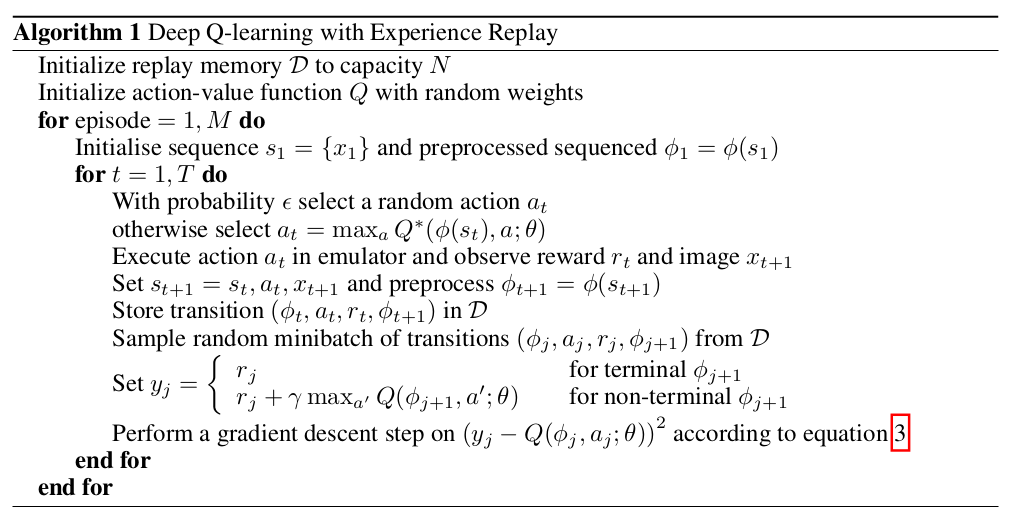
\includegraphics[scale=0.4]{images/DQN_DeepMind_Alg.png}
    \caption{Deep Q Network Algorithm \cite{mnih2013atari}}
    \label{fig:dqn_alg}
\end{figure}

\section{Environments and Experiments}

\subsection{The CartPole Environment}

The first Environment in which the Deep Q Networks are tested is the CartPole Environment, which entails a pole balancing atop a cart which moves in the (frictionless) horizontal plane. The pole is attached to the cart by an unactuated joint. The goal of the environment is to balance the cart on the pole for as long as possible by moving the cart from side to side. The Environment ends when the Cart moves out of (horizontal) bounds (+/- 2.4 units from the centre of the environment) or if the pole falls more than 12 degrees from the centre. The Environment can also terminate if the reward reaches 500.  

\begin{figure}[H]
    \centering
    \includegraphics[scale=0.5]{images/cart_pole.jpeg}
    \caption{The CartPole Environment}
    \label{fig:cartpole}
\end{figure}

\subsubsection{Random Strategy}

To create a base line for obtained reward, the first run of


\section{Conclusions}

\section{Professional Issues}

\section{Self-Assessment}

\newpage
\printbibliography


\end{document}

